%%%%% here is preamble %%%%%

\documentclass{amsart}
\usepackage[english]{babel}
\usepackage[utf8x]{inputenc}
\usepackage{xeCJK}
\usepackage{fontspec}
\usepackage{amsmath}

%%% hyperlink %%%
\usepackage{hyperref}
\hypersetup{
    colorlinks=true,
    linkcolor=blue,
    filecolor=magenta,      
    urlcolor=cyan,
    pdftitle={Overleaf Example},
    pdfpagemode=FullScreen,
    }
%%% hyperlink %%%

%%% code %%%
\usepackage{listings}
\usepackage{xcolor}
\definecolor{codegreen}{rgb}{0,0.6,0}
\definecolor{codegray}{rgb}{0.5,0.5,0.5}
\definecolor{codepurple}{rgb}{0.58,0,0.82}
\definecolor{backcolour}{rgb}{0.95,0.95,0.92}
\lstdefinestyle{mystyle}{
    backgroundcolor=\color{backcolour},   
    commentstyle=\color{codegreen},
    keywordstyle=\color{magenta},
    numberstyle=\tiny\color{codegray},
    stringstyle=\color{codepurple},
    basicstyle=\ttfamily\footnotesize,
    breakatwhitespace=false,         
    breaklines=true,                 
    captionpos=b,                    
    keepspaces=true,                 
    numbers=left,                    
    numbersep=5pt,                  
    showspaces=false,                
    showstringspaces=false,
    showtabs=false,                  
    tabsize=2
}
\lstset{style=mystyle}
%%% code %%%

%%% chinese %%%
\setCJKmainfont{NotoSerifTC-VariableFont_wght.ttf}
%%% chinese %%%

%%% style(margin)%%%
\usepackage
[
    a4paper,
    margin = 2.5cm
]
{geometry}
%%% style(margin)%%%

%%% insert pdf %%%
\usepackage{pdfpages}
%%% insert pdf %%%

%%%%% here is preamble %%%%%

\setlength{\topmargin}{-18mm}
\title{\textbf{Applications of Transition Matrices in Various Recursive Models}}
\author{林士紘、張恩睿、李彥霆、林秉毅、葉宥均}


\begin{document}
\begin{abstract}
    This report investigates the use of transition matrices to solve specific recursive relations, offering a more efficient alternative to traditional Dynamic Programming (DP) approaches for certain problems. By deriving the transition matrices and applying fast matrix exponentiation, we aim to reduce computational complexity. We compare the efficiency of these two methods through theoretical analysis and experimental results, examining whether actual computation times align with the predicted complexities. Our findings demonstrate the potential of transition matrices in optimizing the computation of high-order recurrences, particularly for large-scale problems.
\end{abstract}
\maketitle
\pagestyle{plain}
\pagenumbering{arabic}
\section{Introduction}

\section{Materials and Methods}
\subsection{Materials}

Pen, paper, computer, C++, brains, curiosity for Linear Algebra.

\subsection{Methods}

From the Rail problem, we derived the recurrence relation and its transition matrix.
Then, we implemented recursive functions, DP, and fast matrix exponentiation to compare their computation times across different values of $N$.

\section{Result}

Belowing are the graphs of computation time vs. $N$ for each methods:
\begin{enumerate}
    \item \textbf{Recursive functions} : Execution time grows exponentially.
    \item \textbf{Time complexity $O(N^2)$ DP (hereafter referred to as DP-1)} : Execution time grows quadratically.
    \item \textbf{Time complexity $O(N)$ DP (hereafter referred to as DP-2)} : Execution time grows linearly.
    \item \textbf{Fast matrix exponentiation} : Execution time is roughly constant.
\end{enumerate}

\section{Discussion}

Comparison of the time taken by each method within a specific range of $N$:

Notice that due to the significant differences in execution efficiency among the four methods, it is difficult to compare them directly for the same range of $N$. 
Therefore, we will discuss them in segments based on different ranges of $N$ and select appropriate methods (two or more) for comparison.

\begin{enumerate}
    \item \textbf{When $N \leq 40000$}: 
    
    As shown in the figure below, the time taken by DP-2 grows quadratically, reaching approximately 7000ms at \(N=40000\). In contrast, the time taken by DP-1 and matrix exponentiation methods remains relatively small.
    \item \textbf{When $N \leq 10^7$}:
    
    As shown in the figure below, the time taken by DP-1 grows linearly, reaching approximately 1 second at \(N=4 \times 10^7\). In this range, the matrix exponentiation method remains roughly constant and takes less time than DP-1.

    \item \textbf{When $N \leq 10^{400}$}:
    
    In this very large range of numbers, the time taken by matrix exponentiation grows linearly with \( \log N \), reaching approximately 5000ms at \(N = 10^{400}\).
\end{enumerate}

\section{Conclusion}

\begin{enumerate}
    \item If the \(n\)-th term of a recurrence relation is a linear combination of the previous \(k\) terms, with constant coefficients (such as the Fibonacci sequence), it can always be represented by a \(k \times k\) transition matrix and accelerated using matrix exponentiation.
    \item From the recurrence derived in the Rail problem, we can see that although some recurrences initially do not take the form of a linear combination of previous terms, after simplification, they can still be rewritten as a linear combination of the previous \(k\) terms with constant coefficients, and can be handled similarly to (1) as described above.
    \item From the result graph, it can be observed that transforming the recurrence from its function form to matrix exponentiation significantly improves computational efficiency. The size of \(N\) that can be calculated within a fixed amount of time is roughly on the order of hundreds of powers of 10!
\end{enumerate}

\section{Reference}
\newpage
\renewcommand{\appendixname}{}%
\appendix
\pagenumbering{roman}
\section{Contribution}
\begin{itemize}
    \item []\textbf{113550002} 撰寫遞迴code、繪製內容圖片、製作書面報告、上台發表
    \item []\textbf{113550007} 撰寫dp、矩陣快速冪code、結論公式推導證明、上台發表
    \item []\textbf{113550018} 上影片字幕、上台發表
    \item []\textbf{113550159} code執行與生成結果、製作結果圖表、撰寫書面報告內容、上台發表
    \item []\textbf{113550179} 數據統整、製作影片、製作簡報、撰寫影片講稿、上台發表
\end{itemize}


\section{Rail}
\label{rail}
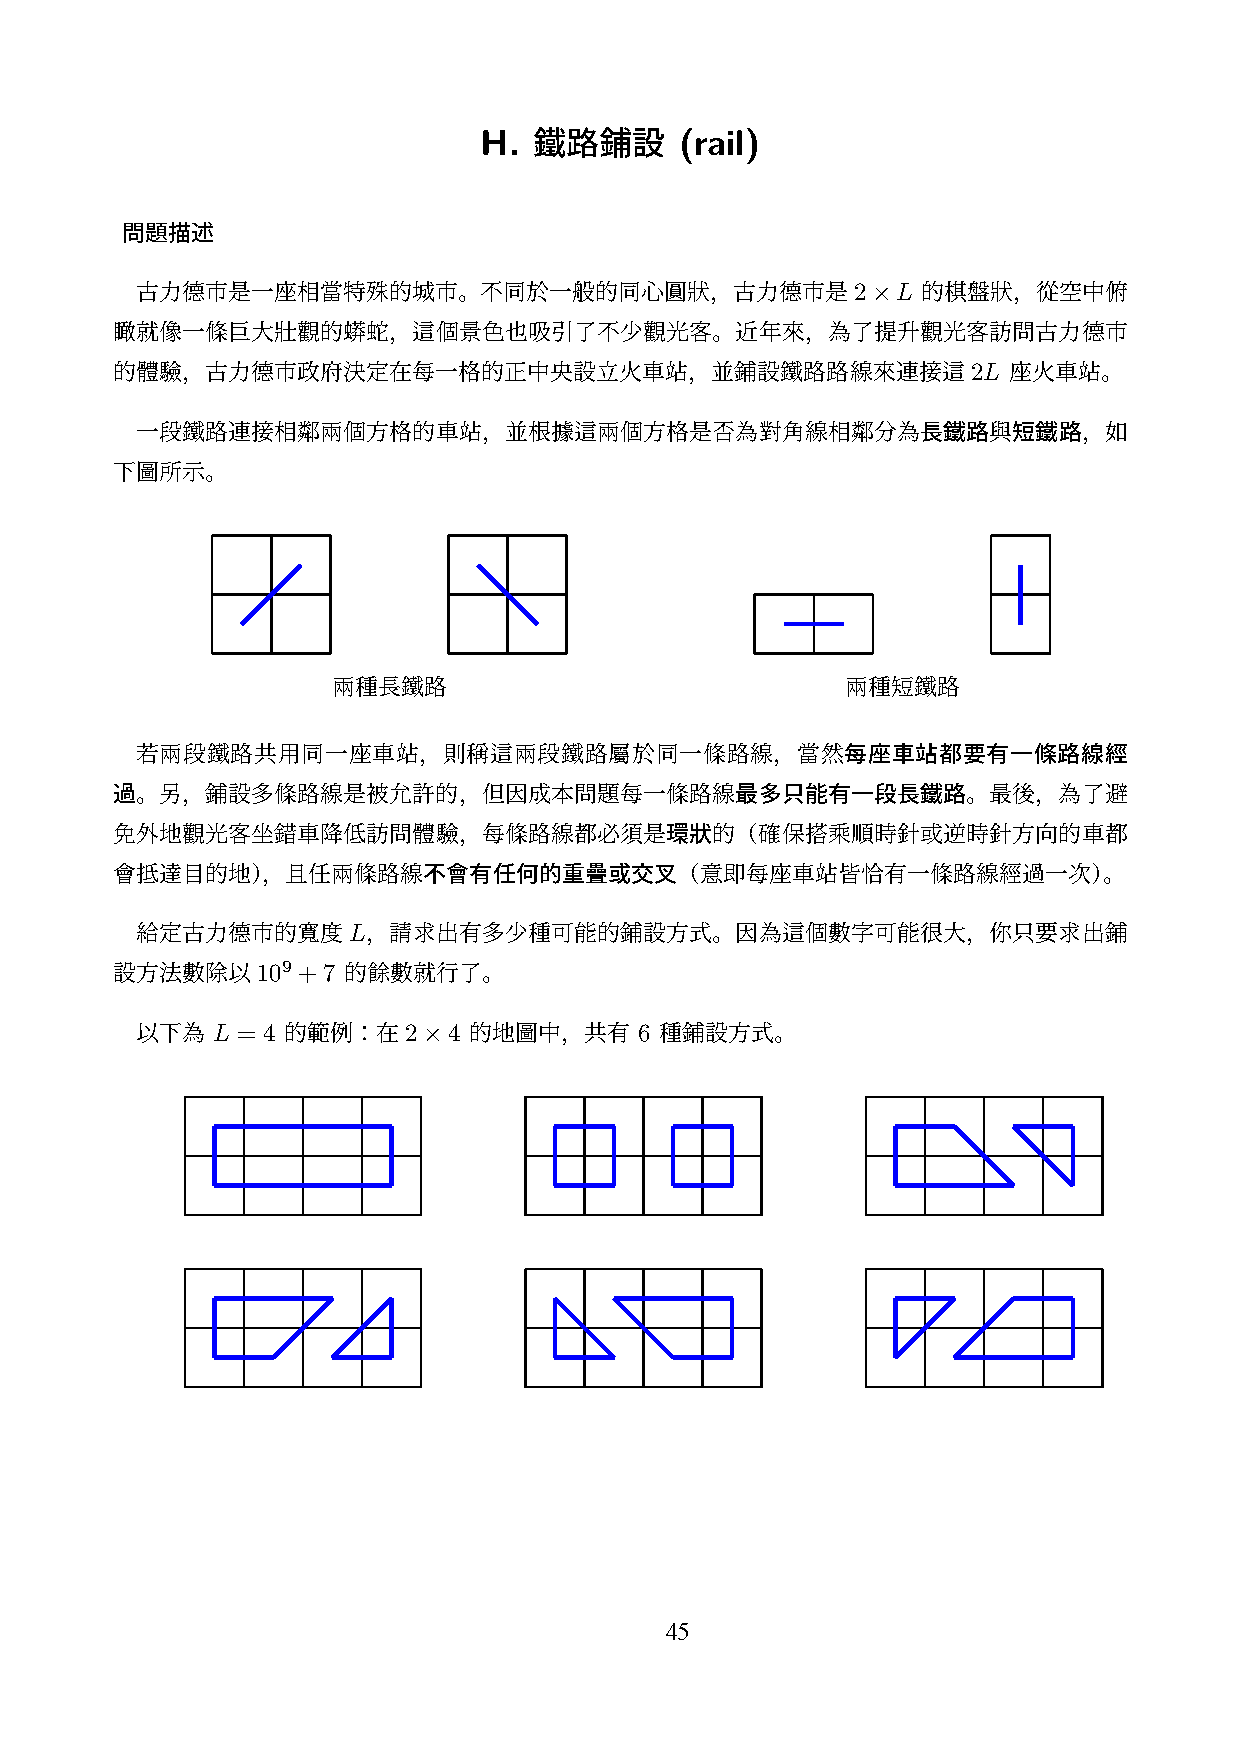
\includepdf[pages=-]{appendices/rail.pdf}

\section{Induction for the Transition Matrix of Rail}
\label{induction for Rail}

\subsection{Induction to recursive formula} 

\section{Code for Fibonacci}
\label{Fibonacci Code}
\subsection{Using Recursion}
\lstinputlisting[language=C++]{appendices/fibonacci_recursion.cpp}

\subsection{Using DP}
\lstinputlisting[language=C++]{appendices/fibonacci.cpp}

\subsection{Using Fast Matrix Power}
\lstinputlisting[language=C++]{appendices/fibonacci_bignum_2.cpp}

\section{Code for Rail}
\label{Rail Code}
\subsection{Using Recursion}
\lstinputlisting[language=C++]{appendices/rail_recursion.cpp}
\subsection{Using DP}
\lstinputlisting[language=C++]{appendices/rail.cpp}
\subsection{Using Fast Matrix Power}
\lstinputlisting[language=C++]{appendices/rail_bignum.cpp}
\end{document}